
\documentclass [12pt,letterpaper]{exam}
\usepackage{amsmath, amsthm, amsfonts, amssymb, amscd}
\usepackage{lipsum}
\usepackage{type1cm}
\usepackage{graphicx}
\usepackage{float}
\usepackage{listings}
\usepackage{color}
\definecolor{mygreen}{RGB}{28,172,0} % color values Red, Green, Blue
\definecolor{mylilas}{RGB}{170,55,241}

%\pagestyle{plain}

\oddsidemargin  0.0in
\evensidemargin 0.0in
\textwidth      6.0in
\headheight     0.0in
\topmargin      0.0in
\textheight     9.0in

\header{ECSE-404}{Control Systems}{December 7, 2016}

\newcounter{count}

%%%%%%%%%%%%%%%%%%%%%%%%%%%%%%%%%%%%%%%%%%%%%%%%%%%%%%%%%%%%%%%%%%%%%%%%%%%%%%%%%%%%%%%%%%%%%%%%%%%%
\begin{document}
\newpage
\tableofcontents
\newpage
%%%%%%%%%%%%%%%%%%%%%%%%%%%%%%%%%%%%%%%%%%%%%%%%%%%%%%%%%%%%%%%%%%%%%%%%%%%%%%%%%%%%%%%%%%%%%%%%%%%%

\lstset{language=Matlab,%
    %basicstyle=\color{red},
    breaklines=true,%
    morekeywords={matlab2tikz},
    keywordstyle=\color{blue},%
    morekeywords=[2]{1}, keywordstyle=[2]{\color{black}},
    identifierstyle=\color{black},%
    stringstyle=\color{mylilas},
    commentstyle=\color{mygreen},%
    showstringspaces=false,%without this there will be a symbol in the places where there is a space
    numbers=left,%
    numberstyle={\tiny \color{black}},% size of the numbers
    numbersep=9pt, % this defines how far the numbers are from the text
    emph=[1]{for,end,break},emphstyle=[1]\color{red}, %some words to emphasise
    %emph=[2]{word1,word2}, emphstyle=[2]{style},    
}
%%%%%%%%%%%%%%%%%%%%%%%%%%%%%%%%%%%%%%%%%%%%%%%%%%%%%%%%%%%%%%%%%%%%%%%%%%%%%%%%%%%%%%%%%%%%%%%%%%%%
\noindent
\section{Abstract}
The problem of stabilizing inverted pendulum is a classic problem in control systems. There has been many detailed studies regarding this topic. This project goal is to explore and discuss possible problems and analyses revolving around the problem of stabilization of an inverted pendulum with one degree of freedom. The project will derive the system equation from classical mechanics and discuss the properties and characteristics of the derived system within the scope of basic control theory. Specifically, linearization, observability, controllability and analysis of transfer function will be discussed. Finally, the project delineates several applicable controllers for the derived system: the pole-placement based controller, the PID controller and the linear quadratic regulator controller.
\newpage

\section{Introduction}
\subsection{System overview}
The physical system is described using the following figure:
\begin{figure}[H]
  \centering
    \includegraphics[width=8cm, height=8cm]{system_diagram} 
  \caption{Inverted pendulum system with one degree of freedom}
  \label{fig:system_diagram}
\end{figure}

The following parameters are considered in the system:
\begin{itemize}
    \item Mass of card $M$
    \item Mass of object at the top of weightless rod $m$
    \item Length of rod $l$
    \item Angle between the rod and y axis $\theta$
    \item Force applied on the cart $F$
    \item Distance between cart and y axis $x$
\end{itemize}

\subsection{Control system objectives}
The objective of the controller designed for this system is to have the mass at the top of the rod kept balanced. That is, the cart has to control the rod by its movement so that the rod aligns itself perpendicular to the ground on which the cart is moving. At such point, the system will also have to ensure that the velocity of the cart is zero to maintain the stability of the mass at any time after that.

The following figure visualizes the system achieving the objective:
\begin{figure}[H]
  \centering
    \includegraphics[width=10cm, height=8cm]{equilibrium_system_diagram} 
  \caption{Inverted pendulum system at objective point}
  \label{fig:equilibrium_system_diagram}
\end{figure}

This implies that the following conditions hold at system stable point:
\begin{align}
\begin{cases}
\theta = 0 \\
\dot{x} = 0
\end{cases}
\end{align}

\newpage
\section{System derivation}
\subsection{Motor modelling}
The force $F$ input into the system can be modelled as coming from a motor. This section describes modelling of an armature controlled DC motor. The following figure from the lecture describes the circuit controlling the motor and the external load with inertia and damping.
\begin{figure}[H]
  \centering
    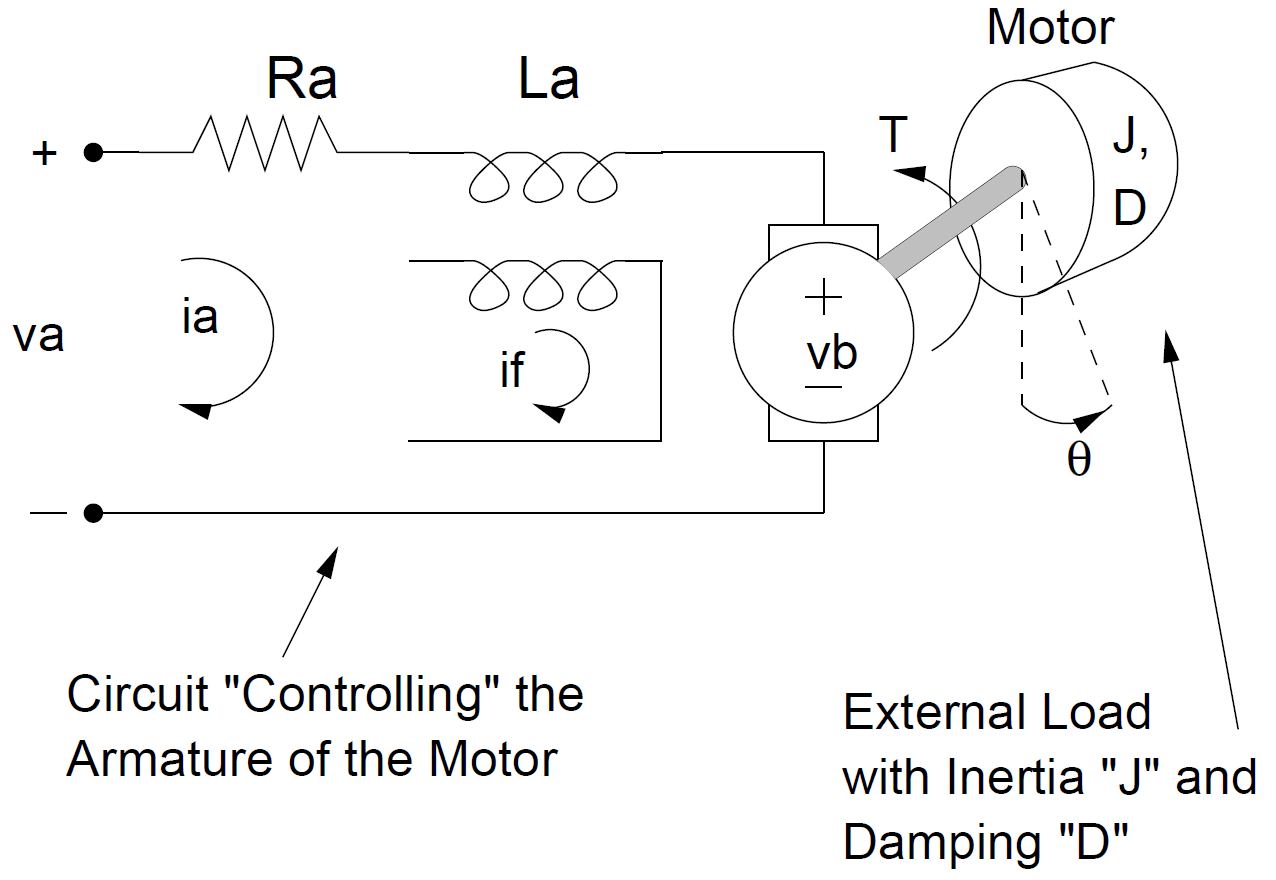
\includegraphics[width=10.15cm, height=7cm]{motor_diagram} 
  \caption{Armature controlled motor modelling}
  \label{fig:motor_diagram}
\end{figure}

The motor is modelled with the following parameters:
\begin{itemize}
    \item $v_a$: voltage externally applied to armature
    \item $R_a$: resistance of armature control circuit
    \item $L_a$: inductance of armature control circuit
    \item $i_a$: current of armature control circuit
    \item $i_f$: emf field (assumed constant)
    \item $v_b$: back emf caused by rotational motion of armature
    \item $T$: torque produced by motor
    \item $\theta$: angular position (displacement) of motor shaft
    \item $K_m$: motor torque constant
    \item $K_b$: back emf constant
\end{itemize}

Using physical laws:
\begin{align}
& T(t) = K_mi_a(t)
\end{align}

The torque due to damping opposes the motion:
\begin{align}
& J\ddot{\theta}(t) = T(t) - D\dot{\theta}(t) \\
& v_b(t) = K_b\frac{d}{dt}\theta(t)
\end{align}

Using KVL:
\begin{align}
& v_a(t) = R_ai_a(t) + L_a\frac{di_a}{dt} + v_b(t)
\end{align}

Solving for $v_a$ yields:
\begin{align}
\begin{split}
& v_a(t) = R_a\bigg(\frac{J}{K_m}\frac{d^2}{dt^2}\theta(t) + \frac{D}{K_m}\frac{d}{dt}\theta(t)\bigg) + L_a\bigg(\frac{J}{K_m}\frac{d^3}{dt^3}\theta(t) + \frac{D}{K_m}\frac{d^2}{dt^2}\theta(t)\bigg) + K_b\frac{d}{dt}\theta(t) \end{split} \\
\begin{split}
& v_a(t) = \frac{L_aJ}{K_m}\frac{d^3}{dt^3}\theta(t) + \bigg(\frac{R_aJ + DL_a}{K_m}\bigg)\frac{d^2}{dt^2}\theta(t) + \bigg(\frac{R_aD}{K_m} + K_b\bigg)\frac{d}{dt}\theta(t)
\end{split}
\end{align}

The required initial conditions are then $\theta(0), \frac{d\theta}{dt}(0), \frac{d^2\theta}{dt^2}(0)$. To simplify the model, we choose the third condition to be zero, leading to the simplification of the equation for $v_a$:

\begin{align}
\int_{0}^{t} v_a(\tau) d\tau = \frac{L_aJ}{K_m}\frac{d^2}{dt^2}\theta(t) + \bigg(\frac{R_aJ + DL_a}{K_m}\bigg)\frac{d}{dt}\theta(t) + \bigg(\frac{R_aD}{K_m} + K_b\bigg)\theta(t)
\end{align}

\subsection{Non-linear system}
With the setup as above, we have the following generalized coordinates:
\begin{align}
& \mbox{Generalized coordinates: } q = [q_1, q_2] = [x, \theta]^T \\
& \mbox{Horizontal position of mass: } x + lsin(\theta) \\
& \mbox{Vertical position of mass: } lcos(\theta)
\end{align}

The total kinetic energy of mass is
\begin{align} 
& T = \frac{1}{2}M\dot{x}^2 + \frac{1}{2}m\bigg[\bigg(\frac{d}{dt}(x + lsin(\theta))\bigg)^2 + \bigg(\frac{d}{dt}(lcos(\theta))\bigg)^2\bigg] \\
& = \frac{1}{2}M\dot{x}^2 + \frac{1}{2}m\bigg[(\dot{x} + l\dot{\theta}cos(\theta))^2 + (-l\dot{\theta}sin(\theta))^2\bigg]
\end{align}

The potential energy of mass is
\begin{align} 
& V = V_o + mglcos(\theta)
\end{align}

where $V_o$ \mbox{ is the potential energy of m for } $\theta = 90^o$.

The Lagrange function is:

\begin{align}
& L = \frac{1}{2}M\dot{x}^2 + \frac{1}{2}m\big[(\dot{x} + l\dot{\theta}cos(\theta))^2 + (l\dot{\theta}sin(\theta))^2\big] - V_o - mglcos(\theta)
\end{align}

We notice that in the described system, F is the only non-conservative force. This means that only the horizontal component of $F$ does work on the system. Therefore, we have the following Lagrange equations:

\begin{align}
& \begin{cases} \frac{d}{dt}\bigg(\frac{\partial L}{\partial \dot{x}}\bigg) - \frac{\partial L}{\partial x} = F \\
\frac{d}{dt}\bigg(\frac{\partial L}{\partial \dot{\theta}}\bigg) - \frac{\partial L}{\partial \theta} = 0
\end{cases}
\end{align}

From here, we compute the derivatives:

\begin{align}
& \frac{\partial L}{\partial \dot{x}} = M\dot{x} + m(\dot{x} + l\dot{\theta}cos(\theta)) \\
& \frac{d}{dt}\bigg(\frac{\partial L}{\partial \dot{x}}\bigg) = M\ddot{x} + m(\ddot{x} + l\ddot{\theta}cos(\theta) - l\dot{\theta}^2sin(\theta) \\
& \frac{\partial L}{\partial x} = 0 \\
\begin{split}
& \frac{\partial L}{\partial \dot{\theta}} = m(\dot{x} + l\dot{\theta}cos(\theta)) + ml^2\dot{\theta}sin^{2}(\theta) = ml\dot{x}cos(\theta) + ml^2\dot{\theta} \\
\end{split} \\
& \frac{d}{dt}\bigg(\frac{\partial L}{\partial \dot{\theta}}\bigg) = ml\ddot{x}cos(\theta) - ml\dot{\theta}\dot{x}sin(\theta) + ml^2\ddot{\theta} \\
\begin{split}
& \frac{\partial L}{\partial \theta} = -m(\dot{x} + l\dot{\theta}cos(\theta))l\dot{\theta}sin(\theta) + ml^2\dot{\theta}^2sin(\theta)cos(\theta) + mglsin(\theta) \\
& = -ml\dot{\theta}\dot{x}sin(\theta) + mglsin(\theta)
\end{split}
\end{align}

Substituting this back into the Lagrange equations above yields:

\begin{align}
\begin{cases}
(M + m)\ddot{x} + ml\ddot{\theta}cos(\theta) - ml\dot{\theta}^2sin(\theta) = F \\
ml\dot{x}cos(\theta) - ml\dot{\theta}\dot{x}sin(\theta) + ml^2\ddot{\theta} + ml\dot{\theta}\dot{x}sin(\theta) - mglsin(\theta) \\
= -ml(\ddot{x}cos(\theta) + l\ddot{\theta} -gsin(\theta)) = 0
\end{cases}
\end{align}

From here, we can derive the final non-linear dynamical model:

\begin{align}
\begin{cases}
(M + m)\ddot{x} + ml\ddot{\theta}cos(\theta) - ml\dot{\theta}^2sin(\theta) = F \\
\ddot{x}cos(\theta) + l\ddot{\theta} -gsin(\theta) = 0
\end{cases}
\end{align}

The following initial conditions are therefore required:
\begin{align}
x(0), \dot{x}(0), \theta(0), \dot{\theta}(0)
\end{align}

\subsection{System state space representation}
Using the dynamical model derived in the previous section, we have the following observations:

\begin{itemize}
    \item $l$ and $g$ are constants
    \item $x$, $\theta$, $\dot{x}$, and $\dot{\theta}$ are system states
    \item $x$ and $\theta$ are output variables
    \item $F$ is the system input
\end{itemize}

Using these observations, we can re-define the system variables:
\begin{align}
\begin{cases}
x_1 = x \\
x_2 = \theta \\
x_3 = \dot{x} \\
x_4 = \dot{\theta} \\
y_1 = x_1 \\
y_2 = x_2 \\
u_1 = F
\end{cases}
\end{align}

Using the newly defined variables in the model, we have
\begin{align}
\begin{cases}
(M + m)\dot{x_3} + ml\dot{x_4}cos(x_2) - mlx_4^2sin(x_2) = u_1 \\
\dot{x_3}cos(x_2) + lx_4 - gsin(x_2) = 0
\end{cases}
\end{align}

Solving for $x_3$ and $x_4$, together with trivial observation that $\dot{x_1} = x_3$ and $\dot{x_2} = x_4$, we have the state space form of the system:
\begin{align}
\begin{cases}
\dot{x_1} = x_3 \\
\dot{x_2} = x_4 \\
\dot{x_3} = \frac{u_1 + mlx_4^2sin(x_2) - mgsin(x_2)cos(x_2)}{M + m(1 - cos^{2}(x_2)} \\
\dot{x_4} = \frac{-u_1cos(x_2) - mlx_4^2sin(x_2)cos(x_2) + (M + m)gsin(x_2)}{l\big[M + m(1 - cos^{2}(x_2)\big]}
\end{cases}
\end{align}

\subsection{Linearization of non-linear system}
Given the objective, it is appropriate to linearize the system around its natural equilibrium point, since this point is also the final objective of the controller to drive the system to. Recall that at indeed at the objective, all first derivatives $\dot{x_i}$ are zero:
\begin{align}
\begin{cases}
\dot{x_1} = 0 \\
\dot{x_2} = 0 \\
\dot{x_3} = 0 \\
\dot{x_4} = 0
\end{cases}
\end{align}

Substituting the known values for $x_i$, we have

\begin{align}
\begin{cases}
x_3 = 0 \\
x_4 = 0 \\
\frac{mlx_4^2sin(x_2) - mgsin(x_2)cos(x_2)}{M + m(1 - cos^{2}(x_2)} = 0 \\
\frac{-mlx_4^2sin(x_2)cos(x_2) + (M + m)gsin(x_2)}{l\big[M + m(1 - cos^{2}(x_2)\big]} = 0
\end{cases}
\end{align}

which is equivalent to

\begin{align}
\begin{cases}
x_1 = x_1 \\
x_2 = k\pi \\
x_3 = 0 \\
x_4 = 0
\end{cases}
\end{align}

We choose $x_2 = \theta = 2n\pi$ to achieve the objective mentioned in the first part of the project. Let this vector $x_e = [x_1, 2n\pi, 0, 0]^T$ be the equilibrium vector, then

$A$ matrix is 

\begin{align}
A = \frac{\partial f}{\partial x} =
\begin{bmatrix}
0 & 0 & 1 & 0 \\
0 & 0 & 0 & 1 \\
0 & \frac{\partial f_3}{\partial x_2} & 0 & \frac{2mlx_4sin(x_2)}{M + m(1 - cos^{2}(x_2)} \\
0 & \frac{\partial f_4}{\partial x_2} & 0 & \frac{2mx_4sin(x_2)cos(x_2)}{M + m(1 - cos^{2}(x_2)} \\
\end{bmatrix}_{x = x_e}
\end{align}

where

\begin{align}
& \frac{\partial f_3}{\partial x_2}_{x = x_e} = \frac{-mg}{M} \\
& \frac{\partial f_4}{\partial x_2}_{x = x_e} = \frac{(M + m)g}{lM}
\end{align}

Therefore,

\begin{align}
A = \frac{\partial f}{\partial x} =
\begin{bmatrix}
0 & 0 & 1 & 0 \\
0 & 0 & 0 & 1 \\
0 & \frac{-mg}{M} & 0 & 0 \\
0 & \frac{(M + m)g}{lM} & 0 & 0 \\
\end{bmatrix}
\end{align}

On the other hand,
\begin{align}
B = \frac{\partial f}{\partial u} =
\begin{bmatrix}
0 \\
0 \\
\frac{1}{M + m(1 - cos^{2}(x_2)} \\
\frac{-cos(x_2)}{l\big[M + m(1 - cos^{2}(x_2)\big]} \\
\end{bmatrix}_{x = x_e}
=
\begin{bmatrix}
0 \\
0 \\
\frac{1}{M} \\
\frac{-1}{lM} \\
\end{bmatrix}
\end{align}

Finally, we have the linearized system around the equilibrium point

\begin{align}
\begin{bmatrix}
\delta\dot{x_1} \\
\delta\dot{x_2} \\
\delta\dot{x_3} \\
\delta\dot{x_4} \\
\end{bmatrix}
=
\begin{bmatrix}
0 & 0 & 1 & 0 \\
0 & 0 & 0 & 1 \\
0 & \frac{-mg}{M} & 0 & 0 \\
0 & \frac{(M + m)g}{lM} & 0 & 0 \\
\end{bmatrix} 
\begin{bmatrix}
\delta x_1 \\
\delta x_2 \\
\delta x_3 \\
\delta x_4 \\
\end{bmatrix}
+
\begin{bmatrix}
0 \\
0 \\
\frac{1}{M} \\
\frac{-1}{lM} \\
\end{bmatrix} \delta u
\end{align}


\subsection{Transfer function}

To derive the transfer function, we recall the following state space form of a general linear system discussed in class:

\begin{align}
\begin{cases}
\dot{x} = Ax + Bu \\
y = Cx + Du \\
x(0) = x_o
\end{cases}
\end{align}

Matching the general system with the generalized system above, and consider the outputs $y_1 = x = x_1$ and $y_2 = \theta = x_2 $, we have
\begin{align}
\begin{cases}
\dot{x} = \begin{bmatrix}
0 & 0 & 1 & 0 \\
0 & 0 & 0 & 1 \\
0 & \frac{-mg}{M} & 0 & 0 \\
0 & \frac{(M + m)g}{lM} & 0 & 0 \\
\end{bmatrix} x
+
\begin{bmatrix}
0 \\
0 \\
\frac{1}{M} \\
\frac{1}{lM} \\
\end{bmatrix} u \\
y = \begin{bmatrix}
1 & 0 & 0 & 0 \\
0 & 1 & 0 & 0
\end{bmatrix} x
\end{cases}
\end{align}

which implies
\begin{align}
A = \begin{bmatrix}
0 & 0 & 1 & 0 \\
0 & 0 & 0 & 1 \\
0 & \frac{-mg}{M} & 0 & 0 \\
0 & \frac{(M + m)g}{lM} & 0 & 0 \\
\end{bmatrix} & &
B = \begin{bmatrix}
0 \\
0 \\
\frac{1}{M} \\
\frac{-1}{lM} \\
\end{bmatrix} \\
C = \begin{bmatrix}
1 & 0 & 0 & 0 \\
0 & 1 & 0 & 0
\end{bmatrix} & &
D = 0
\end{align}

We then have the transfer function
\begin{align}
H(s) = C(sI - A)^{-1}B + D = C(sI - A)^{-1}B \\
\Rightarrow H(s) = \begin{bmatrix}
1 & 0 & 0 & 0 \\
0 & 1 & 0 & 0
\end{bmatrix}
\Bigg(sI - \begin{bmatrix}
0 & 0 & 1 & 0 \\
0 & 0 & 0 & 1 \\
0 & \frac{-mg}{M} & 0 & 0 \\
0 & \frac{(M + m)g}{lM} & 0 & 0 \\
\end{bmatrix}
\Bigg)^{-1} \begin{bmatrix}
0 \\
0 \\
\frac{1}{M} \\
\frac{-1}{lM} \\
\end{bmatrix} \\
\Rightarrow H(s) = \begin{bmatrix}
1 & 0 & 0 & 0 \\
0 & 1 & 0 & 0
\end{bmatrix}
\begin{bmatrix}
s & 0 & -1 & 0 \\
0 & s & 0 & -1 \\
0 & \frac{mg}{M} & s & 0 \\
0 & \frac{-(M + m)g}{lM} & 0 & s \\
\end{bmatrix}^{-1} \begin{bmatrix}
0 \\
0 \\
\frac{1}{M} \\
\frac{-1}{lM} \\
\end{bmatrix}
\end{align}

Here $H(s)$ is a 2 x 1 matrix since we only have 2 outputs. To further simplify the transfer function, we let matrix $A$ and $B$ be in this form

\begin{align}
& A = \begin{bmatrix}
0 & 0 & 1 & 0 \\
0 & 0 & 0 & 1 \\
0 & a & 0 & 0 \\
0 & b & 0 & 0 \\
\end{bmatrix} \mbox{where } a = \frac{-mg}{M} \mbox{ and } b = \frac{(M + m)g}{lM} \\
& B = \begin{bmatrix}
0 \\
0 \\
c \\
d \\
\end{bmatrix} \mbox{where } c = \frac{1}{M} \mbox{ and } d = \frac{-1}{lM}
\end{align}

We can then use Matlab to simplify $H(s)$, which gives a surprisingly simple transfer function.

\begin{align}
& H(s) = \begin{bmatrix} 
\frac{c}{s^2} + \frac{ad}{s^4 - bs^2} \\
\frac{d}{s^2 - b}
\end{bmatrix} \\
& \Rightarrow H(s) =\begin{bmatrix} 
\frac{ad - bc + cs^2}{s^2 (s^2 - b)} \\
\frac{d}{s^2 - b}
\end{bmatrix}
\end{align}

For any natural parameter $l$, $m$, and $M$, we have the following properties for $b$ and $d$.
\begin{align}
& b = \frac{(M + m)g}{lM} > 0 \\
& d = \frac{-1}{lM} < 0
\end{align}

Considering the possible zeros of the system, which are roots of $cs^2 + ad - bc = 0 \Leftrightarrow cs^2 = bc - ad$. We observe that 
\begin{align}
bc - ad = \frac{(M + m)g}{lM^2} - \frac{mg}{lM^2} = \frac{Mg}{lM^2} = \frac{g}{lM} > 0
\end{align}
Therefore the above equation has real roots.

Therefore, this transfer function suggests that the system is proper, and has zeros at $s = \pm\sqrt{b - \frac{ad}{c}}$ and poles at $s = \pm b$ and $s = 0$. Unfortunately, it is unstable as the real part of pole $s = b$ is positive.

\subsection{Observability and controllability}
\subsubsection{Observability}

For the system to be observable, the following matrix must have rank $n = 4$:

\begin{align}
\mathcal{O} =
\begin{bmatrix}
C \\
CA \\
CA^2 \\
... \\
CA^{n-1}
\end{bmatrix} ; rank(\mathcal{O}) = 4
\end{align}

We notice that the first column of $A$ contains all zero. Therefore the first column of $A^2$ will also contains all zero. Consequently, the first column of $CA^{k}$ will contain all zero, implying that the first column of $\mathcal{O}$ will only contain zero. This results in the $\mathcal{O}$ having rank of at most $n - 1$. Therefore, the system is unobservable in the derived state space form regardless of the values of the parameters.

\subsubsection{Controllability}

For the system to be controllable, the following matrix must have rank $n = 4$:
\begin{align}
\mathcal{O}^T =
\begin{bmatrix}
B & AB & A^2B & ... & A^{n-1}B \\
\end{bmatrix} ; rank(\mathcal{O}^T) = 4 
\end{align}

To simplify the calculation, we let matrix $A$ and $B$ be in this form

\begin{align}
& A = \begin{bmatrix}
0 & 0 & 1 & 0 \\
0 & 0 & 0 & 1 \\
0 & a & 0 & 0 \\
0 & b & 0 & 0 \\
\end{bmatrix} \mbox{where } a = \frac{-mg}{M} \mbox{ and } b = \frac{(M + m)g}{lM} \\
& B = \begin{bmatrix}
0 \\
0 \\
c \\
d \\
\end{bmatrix} \mbox{where } c = \frac{1}{M} \mbox{ and } d = \frac{-1}{lM}
\end{align}

We then calculate the constituents of $\mathcal{O}^T$
\begin{align}
& A^2 = AA = \begin{bmatrix}
0 & 0 & 1 & 0 \\
0 & 0 & 0 & 1 \\
0 & a & 0 & 0 \\
0 & b & 0 & 0 \\
\end{bmatrix} \begin{bmatrix}
0 & 0 & 1 & 0 \\
0 & 0 & 0 & 1 \\
0 & a & 0 & 0 \\
0 & b & 0 & 0 \\
\end{bmatrix} \\
& \Rightarrow A^2 = \begin{bmatrix}
0 & a & 0 & 0 \\
0 & b & 0 & 0 \\
0 & 0 & 0 & a \\
0 & 0 & 0 & b \\
\end{bmatrix}
\Rightarrow A^3 = \begin{bmatrix}
0 & 0 & 0 & a \\
0 & 0 & 0 & b \\
0 & ab & 0 & 0 \\
0 & b^2 & 0 & 0 \\
\end{bmatrix} \\
& AB = \begin{bmatrix}
0 & 0 & 1 & 0 \\
0 & 0 & 0 & 1 \\
0 & a & 0 & 0 \\
0 & b & 0 & 0 \\
\end{bmatrix} \begin{bmatrix}
0 \\
0 \\
c \\
d \\
\end{bmatrix} = \begin{bmatrix}
c \\
d \\
0 \\
0 \\
\end{bmatrix} \\
& A^2B = \begin{bmatrix}
0 & a & 0 & 0 \\
0 & b & 0 & 0 \\
0 & 0 & 0 & a \\
0 & 0 & 0 & b \\
\end{bmatrix} \begin{bmatrix}
0 \\
0 \\
c \\
d \\
\end{bmatrix} = \begin{bmatrix}
0 \\
0 \\
ad \\
bd \\
\end{bmatrix} \\
& A^3B = \begin{bmatrix}
0 & 0 & 0 & a \\
0 & 0 & 0 & b \\
0 & ab & 0 & 0 \\
0 & b^2 & 0 & 0 \\
\end{bmatrix} \begin{bmatrix}
0 \\
0 \\
c \\
d \\
\end{bmatrix} = \begin{bmatrix}
ad \\
bd \\
0 \\
0 \\
\end{bmatrix}
\end{align}

The interested matrix $\mathcal{C} = \mathcal{O}^T$ will be

\begin{align}
\mathcal{C} = \mathcal{O}^T = \begin{bmatrix}
0 & c & 0 & ad \\
0 & d & 0 & bd \\
c & 0 & ad & 0 \\
d & 0 & bd & 0 \\
\end{bmatrix}
\end{align}

We can observe that the first and the third column will be linearly dependent, and the second and the fourth column will also be linearly dependent only in rare cases where the two following conditions is true
\begin{align}
& \frac{ad}{c} = \frac{bd}{d} \Leftrightarrow ad = bc \\
& \Leftrightarrow \frac{mg}{lM^2} = \frac{(M + m)g}{lM^2} \\
& \Leftrightarrow mg = Mg + mg \Leftrightarrow M = 0 \mbox{ or } g = 0
\end{align}

This is practically impossible since constant $g \approx 9.81$ and mass of cart $M$ is non-negative. Consequently, all columns of this matrix are linear independent regardless of the values of $a$, $b$, $c$ or $d$ (given that they are derived from some practical inverted pendulum setup in real world). Therefore, the system is controllable for all practical parameters.

\subsection{Sample system open loop response}
With the theoretical analysis above, it is essential to visualize a specific open loop system to gain more insight into its operational characteristics. Below is the plots for a sample set of parameters with the code used to generate the plot. This set of parameter will also be used in the later parts of the report.

\begin{align}
\begin{cases}
m = 1.03kg \\
M = 2.5kg \\
l = 0.75m \\
g = 9.81m/s^2 \\
\end{cases}
\end{align}

\begin{figure}[H]
  \centering
    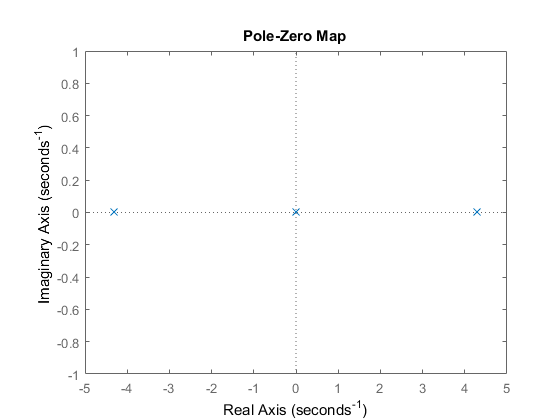
\includegraphics[width=10.15cm, height=7cm]{sample_poles} 
  \caption{Poles of a sample system}
  \label{fig:sample_poles}
\end{figure}

\begin{figure}[H]
  \centering
    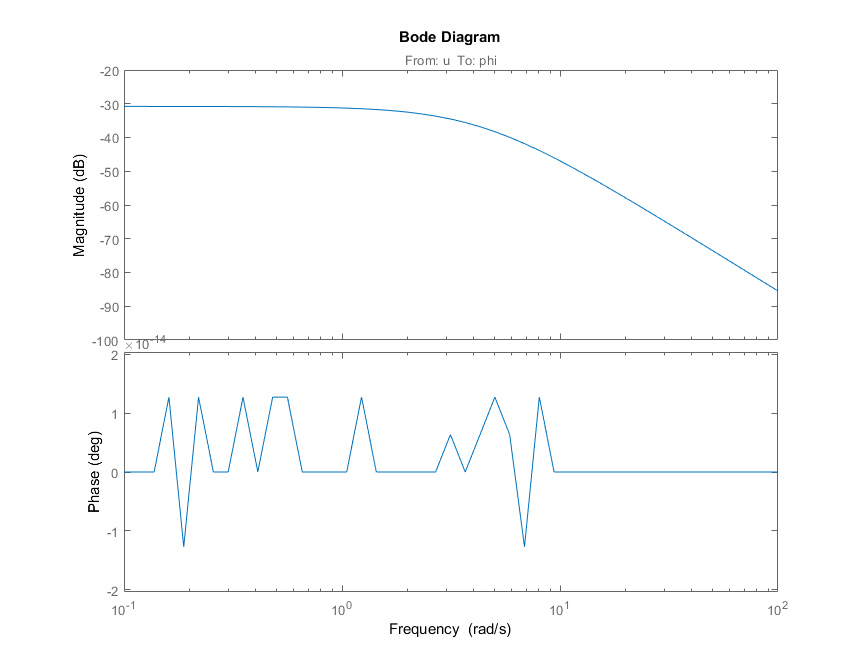
\includegraphics[width=10.15cm, height=7cm]{sample_freq_response} 
  \caption{Frequency response of a sample system}
  \label{fig:sample_freq_response}
\end{figure}

\begin{figure}[H]
  \centering
    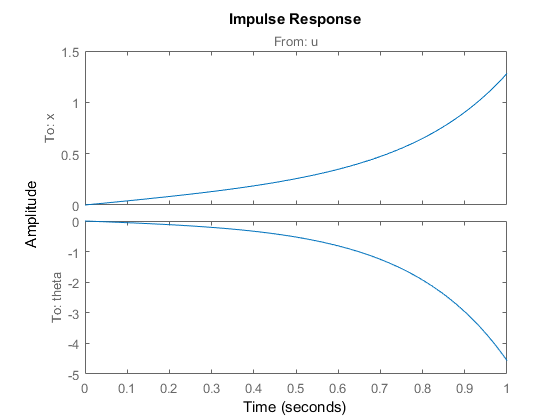
\includegraphics[width=10.15cm, height=7cm]{sample_impulse} 
  \caption{Impulse response of a sample system}
  \label{fig:sample_impulse}
\end{figure}

\lstinputlisting[language=Matlab]{sample_response.m}

\newpage
\section{Controllers}
\subsection{Pole-placement based controller}
\subsubsection{Pole-placement based controller}
This section discusses the design of a closed-loop system with pole-placement controller. The pole-placement based controller suggests an input that is proportional to the internal state of the system. That is, $u = -Kx$ for some constant $K$. The following diagram from the lecture slide describes such setup:
\begin{figure}[H]
  \centering
    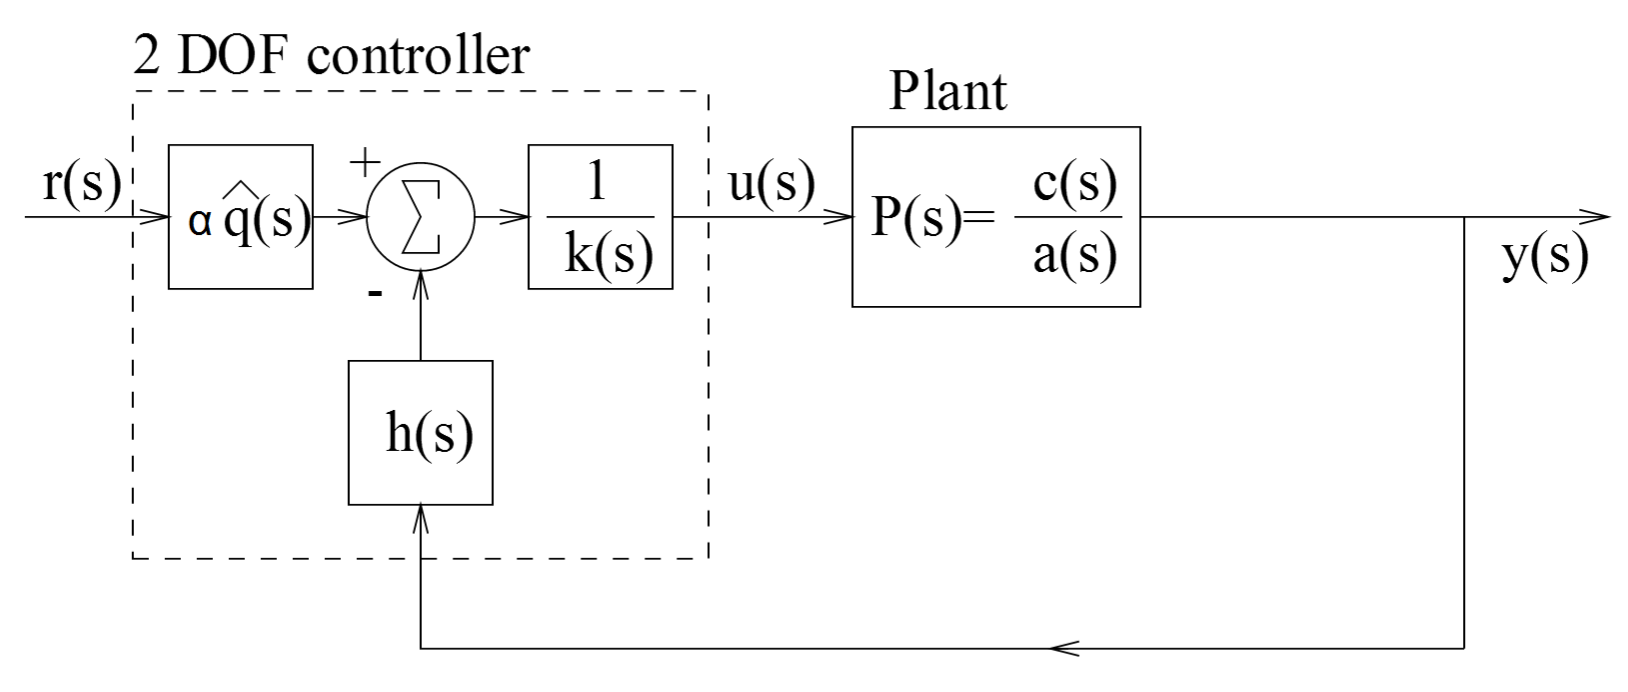
\includegraphics[width=12.76cm, height=5cm]{pl_diagram} 
  \caption{System with pole placement controller}
  \label{fig:pl_diagram}
\end{figure}

To effectively drives the system state, this technique requires the system to be in controllable form, which we already proved above that our system is always controllable. Using this, we can realize the new system with the pole-placement controller:
\begin{align}
\begin{cases}
\dot{x} = Ax + Bu = Ax - BKx = (A - BK)x \\
\dot{y} = Cx + Du = Cx - DKu = (C - DK)x
\end{cases}
\end{align}

There are several salient observations that can be made in the new system. One of which is that the new system characteristic matrices are
\begin{align}
\begin{cases}
A' = A - BK \\
B' = 0
\end{cases}
\end{align}

Therefore, we can utilize our choices of introduced constant matrix $K$ to transform the undesired poles of the original system to new poles that we wish the new system to have. Specifically, we observe that the determinant of $sI - A'$ for the new system being $det(sI - (A - BK))$. Under the last constraint that the degree of the new characteristic equation has to be the same as that of the old one, we can choose our new poles to be $p_1$, $p_2$, ..., $p_n$ and solve the following equation:
\begin{align}
det(sI - (A - BK)) = (s - p_1)(s - p_2)...(s - p_n)
\end{align}

To solve the above equation, we can equate the coefficient at each power of $s$ between the left hand side and the right hand side of the equation, and arrive at a linear system on $n$ equations, which can easily be solved using classic row reduction technique.

\subsubsection{Controllable canonical form}
Given that a system is controllable, we need to transform our original system into controllable canonical form, which is:
\begin{align}
& \dot{x} = \begin{bmatrix}
0 & 1 & 0 & ... & 0 & 0 \\
0 & 0 & 1 & ... & 0 & 0 \\
0 & 0 & 0 & ... & 0 & 0 \\
... \\
0 & 0 & 0 & ... & 0 & 1 \\
-a_0 & -a_1 & -a_2 & ... & -a_{n-2} & -a_{n-1} \\
\end{bmatrix} x + \begin{bmatrix}
0 \\ 0 \\ 0 \\ ... \\ 0 \\1
\end{bmatrix} u\\
& y = \begin{bmatrix}
c_0 & c_1 & c_2 & ... & c_{n-2} & c_{n-1}
\end{bmatrix} x + du
\end{align}

We can transform the original system to its canonical controllable form via the transfer function. Recall that the derived transfer function was:
\begin{align}
H(s) = \frac{d}{s^2 - b}
\end{align}
This is equivalent to the following controllable canonical form:
\begin{align}
& \dot{x} = \begin{bmatrix}
0 & 1 \\
-1 & 0 \\
\end{bmatrix} x + \begin{bmatrix}
0 \\1
\end{bmatrix} u\\
& y = \begin{bmatrix}
d & 0
\end{bmatrix} x + 0u
\end{align}

\subsubsection{First choice of poles}
As an example, using the sample system, our original poles were approximately $s = \pm4.2976$ and $s = 0$. The positive pole is undesirable and should be replaced to improve stability of the system. Using the pole placement controller, we can guess an initial set of new poles as follow:
\begin{itemize}
    \item $p1 = -2$
    \item $p2 = -3$
    \item $p3 = -2 + 0.5i$
    \item $p4 = -2 - 0.5i$
\end{itemize}

This leads to solving for $K = \begin{bmatrix}
k_1 & k_2 & k_3 & k4
\end{bmatrix}$ in the following equation to transform the old poles to the new ones:
\begin{align}
\begin{split}
det(sI - A - BK) = (s + 2)(s + 3)(s + 2 - 0.5i)(s + 2 - 0.5i) \\
= 0.25(s + 2)(s + 3)(4s^2 + 16s + 17)
\end{split}
\end{align}

Using the parameter values from the sample system, we can solve for K:
\begin{align}
K = \begin{bmatrix}
-4.8739 & -95.0034 & -8.6487 & -23.3615
\end{bmatrix}
\end{align}

The following figures (together with the code used to generate it) visualize the results for this choice of poles.
\begin{figure}[H]
  \centering
    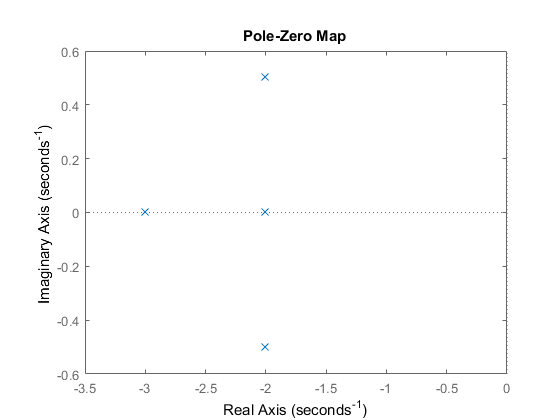
\includegraphics[width=10.15cm, height=7cm]{pl_poles} 
  \caption{Poles of the first choice of pole placement system}
  \label{fig:pl_poles}
\end{figure}

\begin{figure}[H]
  \centering
    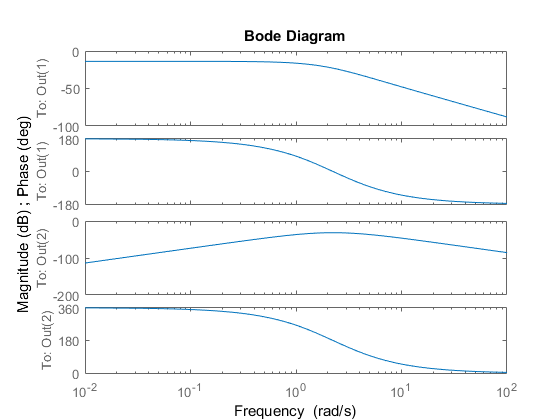
\includegraphics[width=10.15cm, height=7cm]{pl_bode} 
  \caption{Bode plots of the first choice of pole placement system}
  \label{fig:pl_bode}
\end{figure}

\begin{figure}[H]
  \centering
    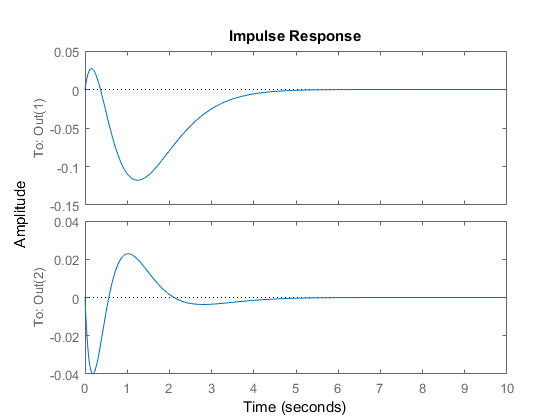
\includegraphics[width=10.15cm, height=7cm]{pl_impulse} 
  \caption{Impulse response of first choice of pole placement system}
  \label{fig:pl_impulse}
\end{figure}

\lstinputlisting[language=Matlab]{pole_placement.m}

\subsubsection{Second choice of poles}
Noticing that there is a significant improvement of system stability over time, we investigate the pole-placement controller with another set of poles. The following diagrams describe the results and the new poles chosen for the second choice. Aiming to improve the performance of the system, we also need to take into account the limitation of the pole-placement method which prevents us from picking poles whose product is greater than $rank(B)$.

\begin{figure}[H]
  \centering
    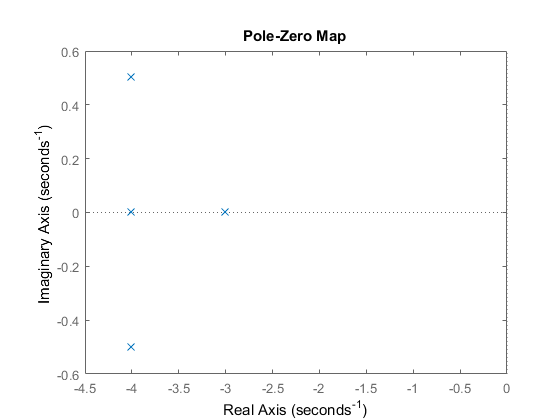
\includegraphics[width=10.15cm, height=7cm]{pl2_poles} 
  \caption{Poles of the second choice of pole placement system}
  \label{fig:pl2_poles}
\end{figure}

\begin{figure}[H]
  \centering
    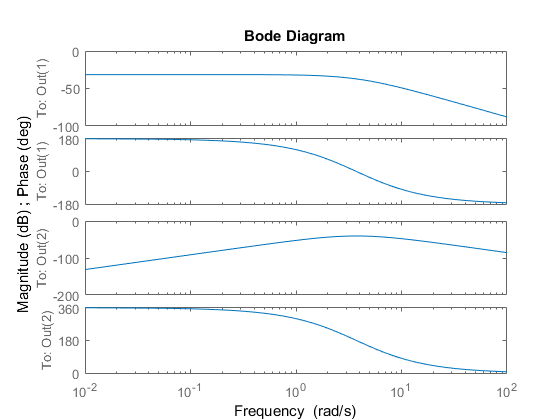
\includegraphics[width=10.15cm, height=7cm]{pl2_bode} 
  \caption{Bode plots of the second choice of pole placement system}
  \label{fig:pl2_bode}
\end{figure}

\begin{figure}[H]
  \centering
    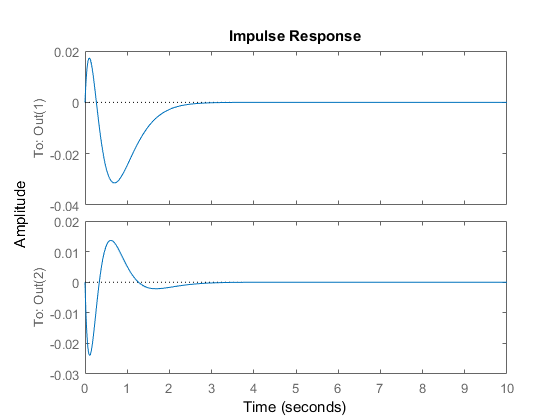
\includegraphics[width=10.15cm, height=7cm]{pl2_impulse} 
  \caption{Impulse response of second choice of pole placement system}
  \label{fig:pl2_impulse}
\end{figure}

\lstinputlisting[language=Matlab]{pole_placement_2.m}

The plots suggest a noticeable improvement of the time taken for the system to reach the objective state (equilibrium). Using the first choice of poles, we reached the objective within approximately $6$ seconds, while with the second choice of poles, we reached the objective within approximately $4$ seconds only. This improvement can be attributed to the choice of poles which have larger real parts, for they were able to bring the system to equilibrium in a shorter amount of time.

\subsubsection{Third choice of poles}
In the third choice of poles, we aim to further improve the results obtained from the second choice of poles above. The following diagrams describe the results and the new poles chosen for the third choice.

\begin{figure}[H]
  \centering
    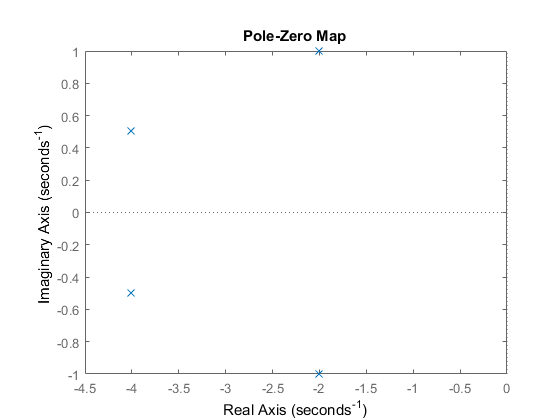
\includegraphics[width=10.15cm, height=7cm]{pl3_poles} 
  \caption{Poles of the third choice of pole placement system}
  \label{fig:pl3_poles}
\end{figure}

\begin{figure}[H]
  \centering
    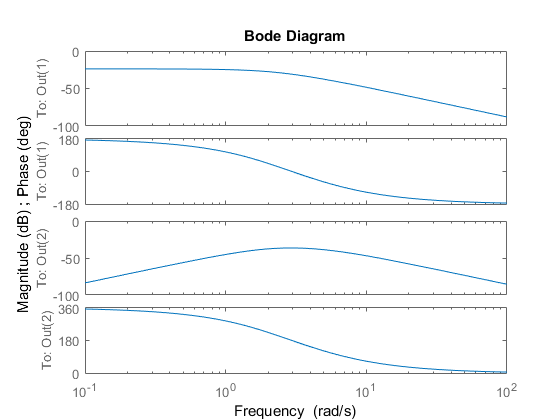
\includegraphics[width=10.15cm, height=7cm]{pl3_bode} 
  \caption{Bode plots of the third choice of pole placement system}
  \label{fig:pl3_bode}
\end{figure}

\begin{figure}[H]
  \centering
    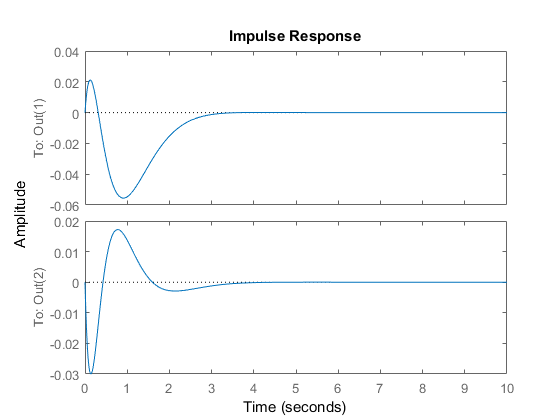
\includegraphics[width=10.15cm, height=7cm]{pl3_impulse} 
  \caption{Impulse response of third choice of pole placement system}
  \label{fig:pl3_impulse}
\end{figure}

\lstinputlisting[language=Matlab]{pole_placement_3.m}

This choice of poles produced very similar results compared to the second choice of poles. There was not much improvement in terms of time required for system to reach stability.


\subsection{PID controller}
\subsubsection{Controller design}
The PID controller is a combination of the Proportional ($P$), Proportional Integral ($PI$) and Proportional Derivative ($PD$) controllers. This combination allows the controller to have great flexibility by having three control parameters to choose. Recalling the three simpler controllers that together forms the PID controller: \\
P controller:
\begin{align}
H_P(s) = K_P \mbox{ for some } K_P > 0
\end{align}
PI controller:
\begin{align}
H_{PI}(s) = \frac{K_I}{s} + K_P \mbox{ for some } K_P > 0 \mbox{ and } K_I > 0
\end{align}
PD controller:
\begin{align}
H_{PD}(s) = K_P(\frac{K_D}{K_P} + 1)
\end{align}

The combination of these three controllers produces the PID controller:
\begin{align}
H^{I}_{PID}(s) = K_P + \frac{K_I}{s} + K_Ds
\end{align}
The visualization of the system is presented in the diagram below.
\begin{figure}[H]
  \centering
    \includegraphics[width=10.52cm, height=3cm]{pid_diagram}
  \caption{Block diagram visualizing the system with pid controller}
  \label{fig:pid_diagram}
\end{figure}

\subsubsection{First choice of K values}
For the first set of K values, we chose the simplest set of parameters: $K_P = K_I = K_D = 1$. The following are the according results and the code used to generate them. We can observe from the plots that the controller fails to drive the system into a stable state, as one of the pole of the overall system has its real part positive, and the impulse response suggests that the system is diverging over time.

\begin{figure}[H]
  \centering
    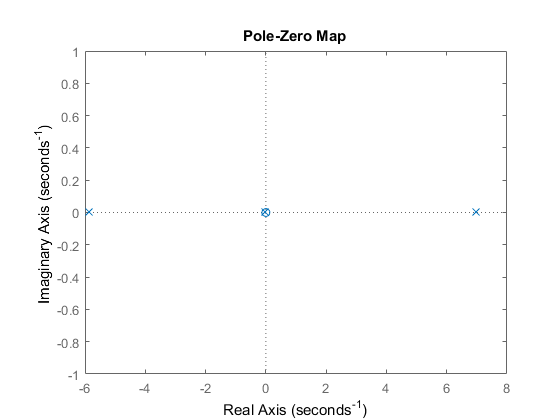
\includegraphics[width=10.15cm, height=7cm]{pid_poles} 
  \caption{Poles of the first choice of pid controller}
  \label{fig:pid_poles}
\end{figure}

\begin{figure}[H]
  \centering
    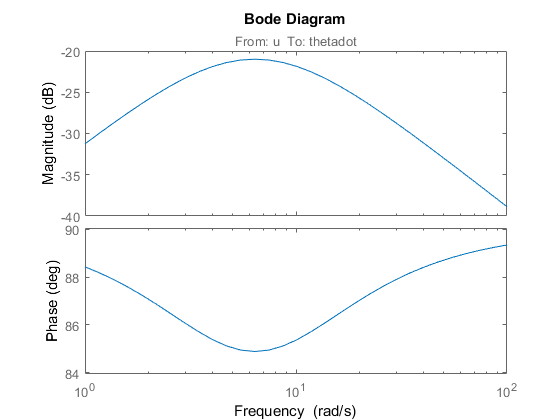
\includegraphics[width=10.15cm, height=7cm]{pid_bode} 
  \caption{Bode plots of the first choice of pid controller}
  \label{fig:pid_bode}
\end{figure}

\begin{figure}[H]
  \centering
    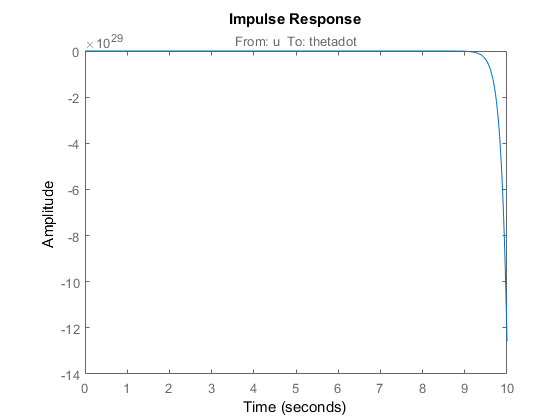
\includegraphics[width=10.15cm, height=7cm]{pid_impulse} 
  \caption{Impulse response of the first choice of pid controller}
  \label{fig:pid_impulse}
\end{figure}

\lstinputlisting[language=Matlab]{pid_controller.m}

\subsubsection{Second choice of $K$ values}
For the second choice of $K$, we selected
\begin{align}
\begin{cases}
K_p = 82 \\
K_i = 1 \\
K_d = 50
\end{cases}
\end{align}
Below are the plots describing the result of this choice of $K$ values, and the code used to generate them. These plot suggest that the controller with these parameters succeeded in stabilizing the system, for the impulse response provides proof of convergence to stability over time.

\begin{figure}[H]
  \centering
    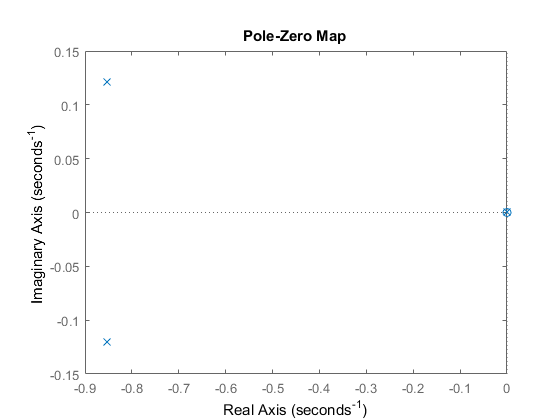
\includegraphics[width=10.15cm, height=7cm]{pid2_poles} 
  \caption{Poles of the second choice of pid controller}
  \label{fig:pid2_poles}
\end{figure}

\begin{figure}[H]
  \centering
    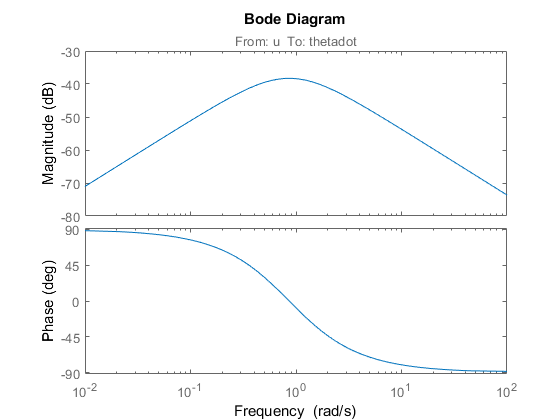
\includegraphics[width=10.15cm, height=7cm]{pid2_bode} 
  \caption{Bode plots of the second choice of pid controller}
  \label{fig:pid2_bode}
\end{figure}

\begin{figure}[H]
  \centering
    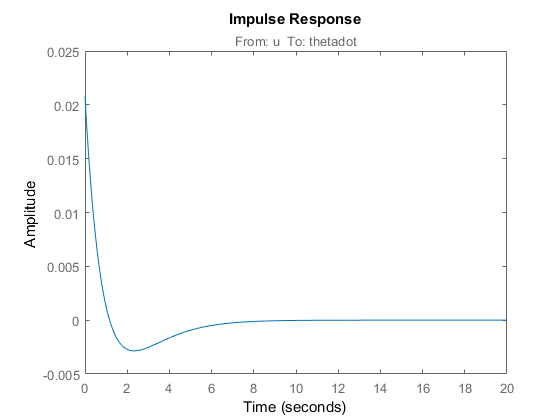
\includegraphics[width=10.15cm, height=7cm]{pid2_impulse} 
  \caption{Impulse response of the second choice of pid controller}
  \label{fig:pid2_impulse}
\end{figure}

\lstinputlisting[language=Matlab]{pid_controller_2.m}

\subsection{Linear quadratic regulator (LQR)}
\subsubsection{Controller design}
The linear quadratic regulartor controller is a modern controller used for multiple input multiple output (MIMO) system. This is recommended over pole placement technique for MIMO system controller design. The LQR controller attempts to minimize the quantity
\begin{align}
\mathcal{I}_{LQR} = \int_{0}^{\infty} [x^T(t)Qx(t) + u^TRu(t)] dx
\end{align}
with $Q = C^TC$ and $R = (R^{\frac{1}{2}})^T(R^{\frac{1}{2}})$ by choosing the feedback $u(x) = Kx$.

\subsubsection{First choice of parameters}
For the first choice of parameters for the LQR controller, we chose the default values deduced from $C^TC$:
\begin{align}
Q = \begin{bmatrix}
1 & 0 & 0 & 0 \\
0 & 0 & 0 & 0 \\
0 & 0 & 1 & 0 \\
0 & 0 & 0 & 0
\end{bmatrix}
\end{align}
Below are the plots of the obtained results and the code used to generate them. These results demonstrates that the LQR controller has been successful in driving the system to stability. However, we can notice that it takes noticeably long (more than 10 seconds) for the system to stabilize.

\begin{figure}[H]
  \centering
    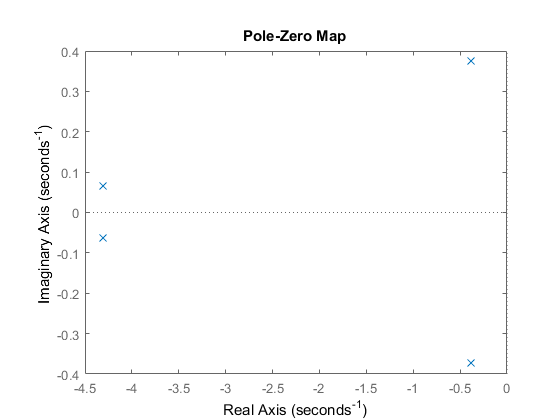
\includegraphics[width=10.15cm, height=7cm]{lqr_poles} 
  \caption{Poles of the first choice of LQR controller}
  \label{fig:lqr_poles}
\end{figure}

\begin{figure}[H]
  \centering
    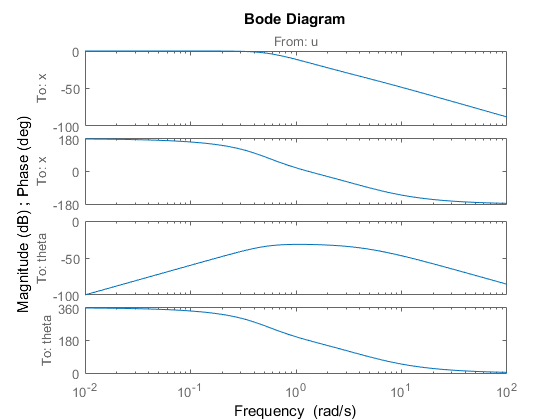
\includegraphics[width=10.15cm, height=7cm]{lqr_bode} 
  \caption{Bode plots of the first choice of pid controller}
  \label{fig:lqr_bode}
\end{figure}

\begin{figure}[H]
  \centering
    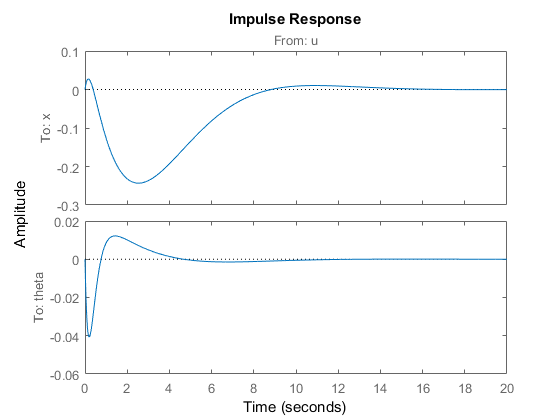
\includegraphics[width=10.15cm, height=7cm]{lqr_impulse} 
  \caption{Impulse response of the second choice of LQR controller}
  \label{fig:lqr_impulse}
\end{figure}

\lstinputlisting[language=Matlab]{lqr_controller.m}

\subsubsection{Second choice of parameters}
We choose another set of parameters in hope of improving the performance of the LQR controller. In particular, the following matrix was used as Q:
\begin{align}
\begin{bmatrix}
500 & 0 & 0 & 0 \\
0 & 10 & 0 & 0 \\
0 & 0 & 1 & 0 \\
0 & 0 & 0 & 0
\end{bmatrix}
\end{align}
The resulting plots and the code used to generate them are presented below. There has been a significant improvement compared to the previous choice of parameters for the LQR controller. Specifically, the time taken for the system to reach stability has been more than halved (under 6 seconds).

\begin{figure}[H]
  \centering
    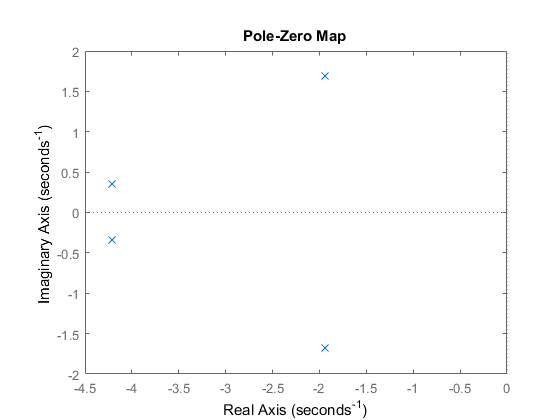
\includegraphics[width=10.15cm, height=7cm]{lqr2_poles} 
  \caption{Poles of the second choice of LQR controller}
  \label{fig:lqr2_poles}
\end{figure}

\begin{figure}[H]
  \centering
    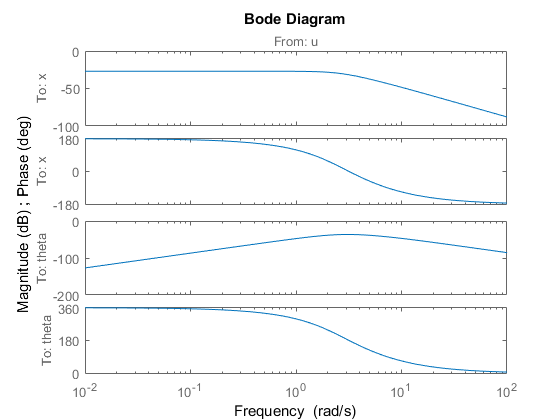
\includegraphics[width=10.15cm, height=7cm]{lqr2_bode} 
  \caption{Bode plots of the second choice of LQR controller}
  \label{fig:lqr2_bode}
\end{figure}

\begin{figure}[H]
  \centering
    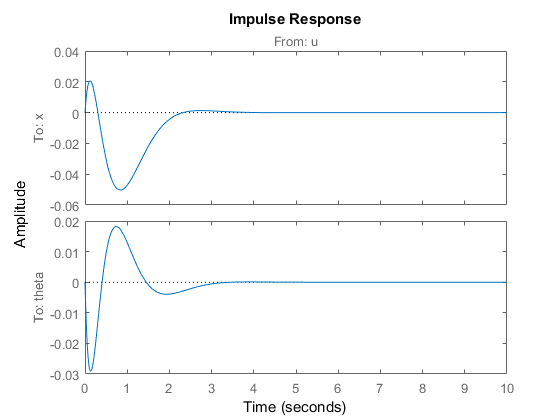
\includegraphics[width=10.15cm, height=7cm]{lqr2_impulse} 
  \caption{Impulse response of the second choice of LQR controller}
  \label{fig:lqr2_impulse}
\end{figure}

\lstinputlisting[language=Matlab]{lqr_controller_2.m}

\newpage
\section{Conclusion}
The project provided great insights into derivation of the classic problem of inverted pendulum in particular, and the basics of control systems in general. The system analyses (i.e. linearization, transfer function analysis, observability and controllability analysis, ...) done on the derived system allowed me to have better exposure experience to application of theoretical results studied in class. The project was very useful as a stimulation for studying the control system subject from a practical point of view, for it has granted precious experience on going beyond the lecture to attain the final goal of understanding of the materials at a higher level. \\
In addition to the theoretical part of the project, simulation of the system together of the designed controllers also provided valuable experience working with Matlab, which has very rich computational packages in general as well as for control systems specifically. This improved my familiarity of the tool and could turn out to be very useful in any research or computational needs I may have in the immediate or a further future.
\newpage


\begin{thebibliography}{9}

\bibitem{lectureslides}
Lecture slides provided by professor Hannah Michalska. 

\bibitem{latexcompanion} 
Michel Goossens, Frank Mittelbach, and Alexander Samarin. 
\textit{The \LaTeX\ Companion}. 
Addison-Wesley, Reading, Massachusetts, 1993.
 
\bibitem{matlabtutorials} 
Control Tutorials for Matlab and Simulink, \\
\texttt{http://ctms.engin.umich.edu/CTMS/index.php?aux=Home}. \\
Accessed 7th December, 2016
\end{thebibliography}
\end{document}
